% Options for packages loaded elsewhere
\PassOptionsToPackage{unicode}{hyperref}
\PassOptionsToPackage{hyphens}{url}
%
\documentclass[
]{article}
\usepackage{amsmath,amssymb}
\usepackage{iftex}
\ifPDFTeX
  \usepackage[T1]{fontenc}
  \usepackage[utf8]{inputenc}
  \usepackage{textcomp} % provide euro and other symbols
\else % if luatex or xetex
  \usepackage{unicode-math} % this also loads fontspec
  \defaultfontfeatures{Scale=MatchLowercase}
  \defaultfontfeatures[\rmfamily]{Ligatures=TeX,Scale=1}
\fi
\usepackage{lmodern}
\ifPDFTeX\else
  % xetex/luatex font selection
\fi
% Use upquote if available, for straight quotes in verbatim environments
\IfFileExists{upquote.sty}{\usepackage{upquote}}{}
\IfFileExists{microtype.sty}{% use microtype if available
  \usepackage[]{microtype}
  \UseMicrotypeSet[protrusion]{basicmath} % disable protrusion for tt fonts
}{}
\makeatletter
\@ifundefined{KOMAClassName}{% if non-KOMA class
  \IfFileExists{parskip.sty}{%
    \usepackage{parskip}
  }{% else
    \setlength{\parindent}{0pt}
    \setlength{\parskip}{6pt plus 2pt minus 1pt}}
}{% if KOMA class
  \KOMAoptions{parskip=half}}
\makeatother
\usepackage{xcolor}
\usepackage[margin=1in]{geometry}
\usepackage{color}
\usepackage{fancyvrb}
\newcommand{\VerbBar}{|}
\newcommand{\VERB}{\Verb[commandchars=\\\{\}]}
\DefineVerbatimEnvironment{Highlighting}{Verbatim}{commandchars=\\\{\}}
% Add ',fontsize=\small' for more characters per line
\usepackage{framed}
\definecolor{shadecolor}{RGB}{248,248,248}
\newenvironment{Shaded}{\begin{snugshade}}{\end{snugshade}}
\newcommand{\AlertTok}[1]{\textcolor[rgb]{0.94,0.16,0.16}{#1}}
\newcommand{\AnnotationTok}[1]{\textcolor[rgb]{0.56,0.35,0.01}{\textbf{\textit{#1}}}}
\newcommand{\AttributeTok}[1]{\textcolor[rgb]{0.13,0.29,0.53}{#1}}
\newcommand{\BaseNTok}[1]{\textcolor[rgb]{0.00,0.00,0.81}{#1}}
\newcommand{\BuiltInTok}[1]{#1}
\newcommand{\CharTok}[1]{\textcolor[rgb]{0.31,0.60,0.02}{#1}}
\newcommand{\CommentTok}[1]{\textcolor[rgb]{0.56,0.35,0.01}{\textit{#1}}}
\newcommand{\CommentVarTok}[1]{\textcolor[rgb]{0.56,0.35,0.01}{\textbf{\textit{#1}}}}
\newcommand{\ConstantTok}[1]{\textcolor[rgb]{0.56,0.35,0.01}{#1}}
\newcommand{\ControlFlowTok}[1]{\textcolor[rgb]{0.13,0.29,0.53}{\textbf{#1}}}
\newcommand{\DataTypeTok}[1]{\textcolor[rgb]{0.13,0.29,0.53}{#1}}
\newcommand{\DecValTok}[1]{\textcolor[rgb]{0.00,0.00,0.81}{#1}}
\newcommand{\DocumentationTok}[1]{\textcolor[rgb]{0.56,0.35,0.01}{\textbf{\textit{#1}}}}
\newcommand{\ErrorTok}[1]{\textcolor[rgb]{0.64,0.00,0.00}{\textbf{#1}}}
\newcommand{\ExtensionTok}[1]{#1}
\newcommand{\FloatTok}[1]{\textcolor[rgb]{0.00,0.00,0.81}{#1}}
\newcommand{\FunctionTok}[1]{\textcolor[rgb]{0.13,0.29,0.53}{\textbf{#1}}}
\newcommand{\ImportTok}[1]{#1}
\newcommand{\InformationTok}[1]{\textcolor[rgb]{0.56,0.35,0.01}{\textbf{\textit{#1}}}}
\newcommand{\KeywordTok}[1]{\textcolor[rgb]{0.13,0.29,0.53}{\textbf{#1}}}
\newcommand{\NormalTok}[1]{#1}
\newcommand{\OperatorTok}[1]{\textcolor[rgb]{0.81,0.36,0.00}{\textbf{#1}}}
\newcommand{\OtherTok}[1]{\textcolor[rgb]{0.56,0.35,0.01}{#1}}
\newcommand{\PreprocessorTok}[1]{\textcolor[rgb]{0.56,0.35,0.01}{\textit{#1}}}
\newcommand{\RegionMarkerTok}[1]{#1}
\newcommand{\SpecialCharTok}[1]{\textcolor[rgb]{0.81,0.36,0.00}{\textbf{#1}}}
\newcommand{\SpecialStringTok}[1]{\textcolor[rgb]{0.31,0.60,0.02}{#1}}
\newcommand{\StringTok}[1]{\textcolor[rgb]{0.31,0.60,0.02}{#1}}
\newcommand{\VariableTok}[1]{\textcolor[rgb]{0.00,0.00,0.00}{#1}}
\newcommand{\VerbatimStringTok}[1]{\textcolor[rgb]{0.31,0.60,0.02}{#1}}
\newcommand{\WarningTok}[1]{\textcolor[rgb]{0.56,0.35,0.01}{\textbf{\textit{#1}}}}
\usepackage{graphicx}
\makeatletter
\def\maxwidth{\ifdim\Gin@nat@width>\linewidth\linewidth\else\Gin@nat@width\fi}
\def\maxheight{\ifdim\Gin@nat@height>\textheight\textheight\else\Gin@nat@height\fi}
\makeatother
% Scale images if necessary, so that they will not overflow the page
% margins by default, and it is still possible to overwrite the defaults
% using explicit options in \includegraphics[width, height, ...]{}
\setkeys{Gin}{width=\maxwidth,height=\maxheight,keepaspectratio}
% Set default figure placement to htbp
\makeatletter
\def\fps@figure{htbp}
\makeatother
\setlength{\emergencystretch}{3em} % prevent overfull lines
\providecommand{\tightlist}{%
  \setlength{\itemsep}{0pt}\setlength{\parskip}{0pt}}
\setcounter{secnumdepth}{-\maxdimen} % remove section numbering
\ifLuaTeX
  \usepackage{selnolig}  % disable illegal ligatures
\fi
\IfFileExists{bookmark.sty}{\usepackage{bookmark}}{\usepackage{hyperref}}
\IfFileExists{xurl.sty}{\usepackage{xurl}}{} % add URL line breaks if available
\urlstyle{same}
\hypersetup{
  pdftitle={Common Loon Data Tidying},
  pdfauthor={Ellie Gabrielson, Will Draxler, Autumn Pauly},
  hidelinks,
  pdfcreator={LaTeX via pandoc}}

\title{Common Loon Data Tidying}
\usepackage{etoolbox}
\makeatletter
\providecommand{\subtitle}[1]{% add subtitle to \maketitle
  \apptocmd{\@title}{\par {\large #1 \par}}{}{}
}
\makeatother
\subtitle{for Statistics Final Project}
\author{Ellie Gabrielson, Will Draxler, Autumn Pauly}
\date{03/12/2024}

\begin{document}
\maketitle

\hypertarget{section}{%
\section{}\label{section}}

\hypertarget{loading-the-packages-and-data}{%
\section{Loading the Packages and
Data}\label{loading-the-packages-and-data}}

\begin{Shaded}
\begin{Highlighting}[]
\FunctionTok{library}\NormalTok{(tidyverse)}
\end{Highlighting}
\end{Shaded}

\begin{verbatim}
## Warning: package 'tidyverse' was built under R version 4.3.3
\end{verbatim}

\begin{verbatim}
## Warning: package 'ggplot2' was built under R version 4.3.2
\end{verbatim}

\begin{verbatim}
## -- Attaching core tidyverse packages ------------------------ tidyverse 2.0.0 --
## v dplyr     1.1.3     v readr     2.1.4
## v forcats   1.0.0     v stringr   1.5.0
## v ggplot2   3.4.4     v tibble    3.2.1
## v lubridate 1.9.2     v tidyr     1.3.0
## v purrr     1.0.2     
## -- Conflicts ------------------------------------------ tidyverse_conflicts() --
## x dplyr::filter() masks stats::filter()
## x dplyr::lag()    masks stats::lag()
## i Use the conflicted package (<http://conflicted.r-lib.org/>) to force all conflicts to become errors
\end{verbatim}

\begin{Shaded}
\begin{Highlighting}[]
\FunctionTok{library}\NormalTok{(lubridate)}
\end{Highlighting}
\end{Shaded}

\hypertarget{loading-data---2023}{%
\section{Loading Data - 2023}\label{loading-data---2023}}

\begin{Shaded}
\begin{Highlighting}[]
\CommentTok{\#2023}
\NormalTok{all\_bird\_untidy\_2023 }\OtherTok{\textless{}{-}} \FunctionTok{read\_csv}\NormalTok{(}\StringTok{"loons\_2023.csv"}\NormalTok{)}
\end{Highlighting}
\end{Shaded}

\begin{verbatim}
## Rows: 577 Columns: 33
## -- Column specification --------------------------------------------------------
## Delimiter: ","
## chr  (19): date, tide, cal, location, species, latitude, longitude, meters_o...
## dbl  (12): year, month, day, tide_percentage, number, temperature, wind_spee...
## lgl   (1): shelter_gradient
## time  (1): time
## 
## i Use `spec()` to retrieve the full column specification for this data.
## i Specify the column types or set `show_col_types = FALSE` to quiet this message.
\end{verbatim}

\begin{Shaded}
\begin{Highlighting}[]
\NormalTok{loons\_2023 }\OtherTok{\textless{}{-}} \FunctionTok{read\_csv}\NormalTok{(}\StringTok{"loons\_2023.csv"}\NormalTok{)}
\end{Highlighting}
\end{Shaded}

\begin{verbatim}
## Rows: 577 Columns: 33
## -- Column specification --------------------------------------------------------
## Delimiter: ","
## chr  (19): date, tide, cal, location, species, latitude, longitude, meters_o...
## dbl  (12): year, month, day, tide_percentage, number, temperature, wind_spee...
## lgl   (1): shelter_gradient
## time  (1): time
## 
## i Use `spec()` to retrieve the full column specification for this data.
## i Specify the column types or set `show_col_types = FALSE` to quiet this message.
\end{verbatim}

\begin{Shaded}
\begin{Highlighting}[]
\CommentTok{\#2024}
\NormalTok{loons\_2024 }\OtherTok{\textless{}{-}} \FunctionTok{read\_csv}\NormalTok{(}\StringTok{"loons\_2024.csv"}\NormalTok{)}
\end{Highlighting}
\end{Shaded}

\begin{verbatim}
## Rows: 775 Columns: 31
## -- Column specification --------------------------------------------------------
## Delimiter: ","
## chr  (19): date, tide, location, species, latitude, behavior, sex, behavior_...
## dbl  (11): number, longitude, meters_offshore, temperature, wind_speed, baro...
## time  (1): time
## 
## i Use `spec()` to retrieve the full column specification for this data.
## i Specify the column types or set `show_col_types = FALSE` to quiet this message.
\end{verbatim}

\hypertarget{tidying-the-data}{%
\section{Tidying the Data}\label{tidying-the-data}}

\hypertarget{exposure}{%
\subsection{Exposure}\label{exposure}}

\begin{Shaded}
\begin{Highlighting}[]
\CommentTok{\#assigning exposure level to locations}
\NormalTok{loons\_2023 }\OtherTok{\textless{}{-}}\NormalTok{ loons\_2023 }\SpecialCharTok{\%\textgreater{}\%} 
  \FunctionTok{mutate}\NormalTok{(}\AttributeTok{shelter\_gradient =} \FunctionTok{case\_when}\NormalTok{(location }\SpecialCharTok{==} \StringTok{"BAR HARBOR PIER"} \SpecialCharTok{\textasciitilde{}} \StringTok{"exposed"}\NormalTok{,}
\NormalTok{                                      location }\SpecialCharTok{==} \StringTok{"SEAL HARBOR BEACH"} \SpecialCharTok{\textasciitilde{}} \StringTok{"moderate"}\NormalTok{,}
\NormalTok{                                      location }\SpecialCharTok{==} \StringTok{"BRACY HARBOR"} \SpecialCharTok{\textasciitilde{}} \StringTok{"moderate"}\NormalTok{,}
\NormalTok{                                      location }\SpecialCharTok{==} \StringTok{"NORTHEAST HARBOR"} \SpecialCharTok{\textasciitilde{}} \StringTok{"moderately\_sheltered"}\NormalTok{,}
\NormalTok{                                      location }\SpecialCharTok{==} \StringTok{"SOMES SOUND"} \SpecialCharTok{\textasciitilde{}} \StringTok{"sheltered"}\NormalTok{,}
\NormalTok{                                      location }\SpecialCharTok{==} \StringTok{"SOUTHWEST HARBOR"} \SpecialCharTok{\textasciitilde{}} \StringTok{"moderately\_sheltered"}\NormalTok{,}
\NormalTok{                                      location }\SpecialCharTok{==} \StringTok{"SEAWALL"} \SpecialCharTok{\textasciitilde{}} \StringTok{"exposed"}\NormalTok{,}
\NormalTok{                                      location }\SpecialCharTok{==} \StringTok{"SEAL COVE"} \SpecialCharTok{\textasciitilde{}} \StringTok{"moderately\_exposed"}\NormalTok{,}
\NormalTok{                                      location }\SpecialCharTok{==} \StringTok{"SAND BEACH"} \SpecialCharTok{\textasciitilde{}} \StringTok{"moderately\_exposed"}\NormalTok{))}
 
\CommentTok{\#releveling the exposure levels from most exposed to least exposed }
\NormalTok{shelter\_factor }\OtherTok{\textless{}{-}} \FunctionTok{fct\_relevel}\NormalTok{(loons\_2023}\SpecialCharTok{$}\NormalTok{shelter\_gradient, }\FunctionTok{c}\NormalTok{(}
                \StringTok{"exposed"}\NormalTok{, }
                \StringTok{"moderately\_exposed"}\NormalTok{,}
                \StringTok{"moderate"}\NormalTok{,}
                \StringTok{"moderately\_sheltered"}\NormalTok{,}
                \StringTok{"sheltered"}\NormalTok{))}

\CommentTok{\#saving a dataset to include only loons and the shelter factor}
\NormalTok{loons\_2023 }\OtherTok{\textless{}{-}}\NormalTok{ loons\_2023 }\SpecialCharTok{\%\textgreater{}\%} 
  \FunctionTok{mutate}\NormalTok{(}\AttributeTok{shelter\_factor =}\NormalTok{ shelter\_factor) }\SpecialCharTok{\%\textgreater{}\%} 
  \FunctionTok{filter}\NormalTok{(species }\SpecialCharTok{==} \StringTok{"COMMON LOON"}\NormalTok{)}

\CommentTok{\#counting how many different exposure observations we have}
\NormalTok{loons\_2023 }\SpecialCharTok{\%\textgreater{}\%} 
  \FunctionTok{count}\NormalTok{(shelter\_factor)}
\end{Highlighting}
\end{Shaded}

\begin{verbatim}
## # A tibble: 5 x 2
##   shelter_factor           n
##   <fct>                <int>
## 1 exposed                 48
## 2 moderately_exposed      33
## 3 moderate                29
## 4 moderately_sheltered    17
## 5 sheltered                4
\end{verbatim}

\hypertarget{changing-chr-variables-to-num}{%
\subsection{\texorpdfstring{Changing \texttt{chr} variables to
\texttt{num}}{Changing chr variables to num}}\label{changing-chr-variables-to-num}}

There are a number of variables within this dataset that are character
variables that should be numeric variables (i.e.~meters\_offshore,
longitude, latitude)

\begin{Shaded}
\begin{Highlighting}[]
\CommentTok{\#Change character numbers to numeric}
\NormalTok{loons\_2023 }\OtherTok{\textless{}{-}}\NormalTok{ loons\_2023 }\SpecialCharTok{\%\textgreater{}\%} 
  \FunctionTok{mutate}\NormalTok{(}\AttributeTok{meters\_offshore =} \FunctionTok{as.numeric}\NormalTok{(meters\_offshore)) }\SpecialCharTok{\%\textgreater{}\%} 
  \FunctionTok{mutate}\NormalTok{(}\AttributeTok{latitude =} \FunctionTok{as.numeric}\NormalTok{(latitude)) }\SpecialCharTok{\%\textgreater{}\%} 
  \FunctionTok{mutate}\NormalTok{(}\AttributeTok{longitude =} \FunctionTok{as.numeric}\NormalTok{(longitude)) }\SpecialCharTok{\%\textgreater{}\%} 
  \FunctionTok{mutate}\NormalTok{(}\AttributeTok{barometer =} \FunctionTok{as.numeric}\NormalTok{(barometer)) }\SpecialCharTok{\%\textgreater{}\%} 
  \FunctionTok{mutate}\NormalTok{(}\AttributeTok{date =} \FunctionTok{as\_date}\NormalTok{(date, }\AttributeTok{format =} \StringTok{"\%m/\%d/\%Y"}\NormalTok{)) }\SpecialCharTok{\%\textgreater{}\%} 
  \FunctionTok{mutate}\NormalTok{(}\AttributeTok{time =}\NormalTok{ hms}\SpecialCharTok{::}\FunctionTok{as\_hms}\NormalTok{(time)) }\SpecialCharTok{\%\textgreater{}\%} 
  \FunctionTok{select}\NormalTok{(}\SpecialCharTok{{-}}\NormalTok{year, }\SpecialCharTok{{-}}\NormalTok{day, }\SpecialCharTok{{-}}\NormalTok{month)}
\end{Highlighting}
\end{Shaded}

\begin{verbatim}
## Warning: There was 1 warning in `mutate()`.
## i In argument: `barometer = as.numeric(barometer)`.
## Caused by warning:
## ! NAs introduced by coercion
\end{verbatim}

\begin{Shaded}
\begin{Highlighting}[]
\FunctionTok{glimpse}\NormalTok{(loons\_2023)}
\end{Highlighting}
\end{Shaded}

\begin{verbatim}
## Rows: 131
## Columns: 31
## $ date               <date> 2023-01-04, 2023-01-04, 2023-01-04, 2023-01-04, 20~
## $ time               <time> 14:20:00, 14:20:00, 14:20:00, 14:20:00, 14:50:00, ~
## $ tide_percentage    <dbl> 0, 0, 0, 0, 0, 0, 0, 0, 50, 50, 50, 60, 60, 60, 60,~
## $ tide               <chr> "LOW", "LOW", "LOW", "LOW", "LOW", "LOW", "LOW", "L~
## $ cal                <chr> "LOW EBB", "LOW EBB", "LOW EBB", "LOW EBB", "LOW", ~
## $ location           <chr> "BAR HARBOR PIER", "BAR HARBOR PIER", "BAR HARBOR P~
## $ species            <chr> "COMMON LOON", "COMMON LOON", "COMMON LOON", "COMMO~
## $ number             <dbl> 1, 1, 1, 1, 1, 1, 1, 1, 1, 1, 1, 1, 1, 1, 1, 1, 1, ~
## $ latitude           <dbl> 44.39161, 44.39124, 44.39107, 44.39105, 44.29530, 4~
## $ longitude          <dbl> -68.20366, -68.20303, -68.20228, -68.20255, -68.239~
## $ meters_offshore    <dbl> 50, 37, 18, 16, 15, 450, 440, 300, 100, 30, 30, 153~
## $ behavior           <chr> "PEERING", "DIVING", "DRIFTING", "DRIFTING", "DIVIN~
## $ behavior_notes     <chr> NA, NA, NA, NA, NA, NA, NA, NA, NA, NA, NA, NA, NA,~
## $ sky_condition      <chr> "CLOUDY, WINDY", "CLOUDY, WINDY", "CLOUDY, WINDY", ~
## $ weather_notes      <chr> NA, NA, NA, NA, NA, NA, NA, NA, NA, NA, NA, NA, NA,~
## $ precipitation      <chr> "NONE", "NONE", "NONE", "NONE", "NONE", "NONE", "NO~
## $ temperature        <dbl> 42.5, 42.5, 42.5, 42.5, 42.7, 42.0, 42.0, 42.0, 32.~
## $ wind_speed         <dbl> 2.0, 2.0, 2.0, 2.0, 2.4, 2.0, 2.0, 2.0, 5.0, 5.0, 5~
## $ wind_direction     <chr> "NNE", "NNE", "NNE", "NNE", "NNE", "NNE", "NNE", "N~
## $ barometer          <dbl> 29.98, 29.98, 29.98, 29.98, 29.98, 29.98, 29.98, 29~
## $ humidity           <dbl> 88, 88, 88, 88, 88, 88, 88, 88, 97, 97, 97, 97, 97,~
## $ cloud_coverage     <dbl> 100, 100, 100, 100, 75, 60, 60, 60, 100, 100, 100, ~
## $ wave_class         <dbl> 1.0, 1.0, 1.0, 1.0, 2.0, 2.0, 2.0, 2.0, 3.0, 3.0, 3~
## $ human_activity     <chr> "CONSTRUCTION", "CONSTRUCTION", "CONSTRUCTION", "CO~
## $ water_activity     <chr> "NONE", "NONE", "NONE", "NONE", "NONE", "NONE", "NO~
## $ shelter_gradient   <chr> "exposed", "exposed", "exposed", "exposed", "modera~
## $ notes              <chr> NA, NA, NA, NA, NA, NA, NA, NA, NA, NA, NA, NA, NA,~
## $ moon_phase         <chr> "WAXING GIBBOUS", "WAXING GIBBOUS", "WAXING GIBBOUS~
## $ overall_abundance  <dbl> 8, 8, 8, 8, 8, 8, 8, 8, 7, 7, 7, 7, 7, 7, 7, 4, 4, ~
## $ specific_abundance <dbl> 4, 4, 4, 4, 1, 3, 3, 3, 3, 3, 3, 3, 3, 3, 1, 1, 2, ~
## $ shelter_factor     <fct> exposed, exposed, exposed, exposed, moderate, moder~
\end{verbatim}

\hypertarget{location}{%
\subsection{Location}\label{location}}

\begin{Shaded}
\begin{Highlighting}[]
\CommentTok{\#determining how many locations we have}
\FunctionTok{unique}\NormalTok{(loons\_2023}\SpecialCharTok{$}\NormalTok{location)}
\end{Highlighting}
\end{Shaded}

\begin{verbatim}
## [1] "BAR HARBOR PIER"   "SEAL HARBOR BEACH" "BRACY HARBOR"     
## [4] "NORTHEAST HARBOR"  "SOMES SOUND"       "SOUTHWEST HARBOR" 
## [7] "SEAWALL"           "SEAL COVE"         "SAND BEACH"
\end{verbatim}

\hypertarget{behavior}{%
\subsection{Behavior}\label{behavior}}

\begin{Shaded}
\begin{Highlighting}[]
\FunctionTok{unique}\NormalTok{(loons\_2023}\SpecialCharTok{$}\NormalTok{behavior)}
\end{Highlighting}
\end{Shaded}

\begin{verbatim}
## [1] "PEERING"     "DIVING"      "DRIFTING"    "MAINTENANCE" "ASHORE"
\end{verbatim}

\begin{Shaded}
\begin{Highlighting}[]
\CommentTok{\#Count occurence of behaviors}
\NormalTok{loons\_2023\_behavior }\OtherTok{\textless{}{-}}\NormalTok{ loons\_2023 }\SpecialCharTok{\%\textgreater{}\%} 
  \FunctionTok{filter}\NormalTok{(species }\SpecialCharTok{==} \StringTok{"COMMON LOON"}\NormalTok{) }\SpecialCharTok{\%\textgreater{}\%} 
  \FunctionTok{group\_by}\NormalTok{(date, behavior, species, tide, tide\_percentage) }\SpecialCharTok{\%\textgreater{}\%} 
  \FunctionTok{count}\NormalTok{(behavior)}

\NormalTok{loons\_2023\_behavior}
\end{Highlighting}
\end{Shaded}

\begin{verbatim}
## # A tibble: 52 x 6
## # Groups:   date, behavior, species, tide, tide_percentage [52]
##    date       behavior    species     tide  tide_percentage     n
##    <date>     <chr>       <chr>       <chr>           <dbl> <int>
##  1 2023-01-04 DIVING      COMMON LOON LOW                 0     4
##  2 2023-01-04 DRIFTING    COMMON LOON LOW                 0     2
##  3 2023-01-04 MAINTENANCE COMMON LOON LOW                 0     1
##  4 2023-01-04 PEERING     COMMON LOON LOW                 0     1
##  5 2023-01-06 DIVING      COMMON LOON MID                50     3
##  6 2023-01-06 DIVING      COMMON LOON MID                60     4
##  7 2023-01-08 DIVING      COMMON LOON HIGH               90     3
##  8 2023-01-08 DRIFTING    COMMON LOON HIGH               90     1
##  9 2023-01-12 DIVING      COMMON LOON LOW                 0     3
## 10 2023-01-12 DIVING      COMMON LOON LOW                10     2
## # i 42 more rows
\end{verbatim}

\begin{Shaded}
\begin{Highlighting}[]
\CommentTok{\#Count the occurrences of behavior of loons}
\FunctionTok{ggplot}\NormalTok{(}\AttributeTok{data =}\NormalTok{ loons\_2023\_behavior, }\AttributeTok{mapping =} \FunctionTok{aes}\NormalTok{(}\AttributeTok{x =}\NormalTok{ behavior)) }\SpecialCharTok{+} 
  \FunctionTok{geom\_bar}\NormalTok{()}
\end{Highlighting}
\end{Shaded}

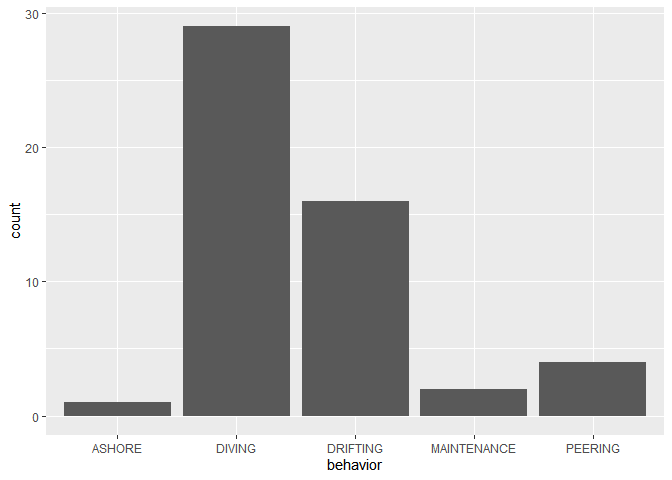
\includegraphics{datatidying_files/figure-latex/behavior-tidying-1.pdf}

\begin{Shaded}
\begin{Highlighting}[]
\CommentTok{\#Count how many low, high, and mid tide observations we have}
\FunctionTok{ggplot}\NormalTok{(}\AttributeTok{data =}\NormalTok{ loons\_2023\_behavior, }\AttributeTok{mapping =} \FunctionTok{aes}\NormalTok{(}\AttributeTok{x =}\NormalTok{ tide)) }\SpecialCharTok{+} 
  \FunctionTok{geom\_bar}\NormalTok{()}
\end{Highlighting}
\end{Shaded}

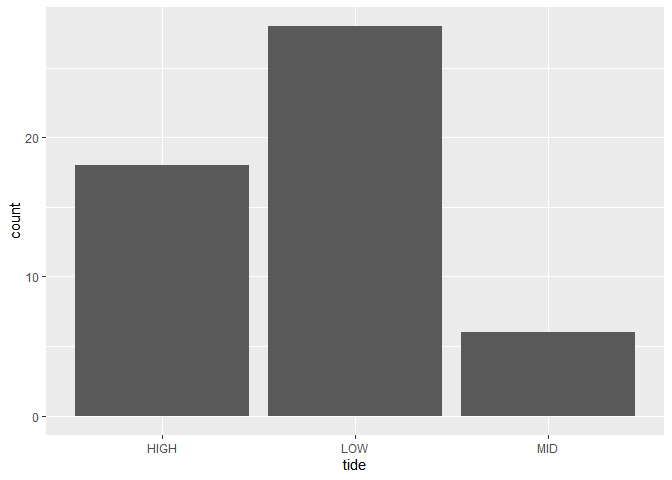
\includegraphics{datatidying_files/figure-latex/behavior-tidying-2.pdf}

\end{document}
